\documentclass{article}

% Language setting
% Replace `english' with e.g. `spanish' to change the document language
\usepackage[english]{babel}
\usepackage{minted}

% Set page size and margins
% Replace `letterpaper' with `a4paper' for UK/EU standard size
\usepackage[letterpaper,top=2cm,bottom=2cm,left=3cm,right=3cm,marginparwidth=1.75cm]{geometry}

% Useful packages
\usepackage{amsmath}
\usepackage{graphicx}
\usepackage[colorlinks=true, allcolors=blue]{hyperref}

\title{ME-489 HOMEWORK 2 REPORT}
\author{Alperen Çalışkan & Ali Taha Akpınar}

\begin{document}
\definecolor{mygray}{rgb}{0.95,0.95,0.95}
\setminted[c]{autogobble=true, frame=lines, framesep=4mm, baselinestretch=1.2,
bgcolor=mygray, fontsize=\footnotesize,linenos=true}
\setminted[latex]{autogobble=true, frame=lines, framesep=4mm, baselinestretch=1.2,
bgcolor=mygray, fontsize=\footnotesize,linenos=true}
\maketitle
\begin{abstract}

This report is a documentation of the ME-489 Homework code. It explains the problem and the methods used for solving the problem. The document also discusses the completed code and its implementation using Paraview. The code itself belongs to the teacher of the class since it was originally made by him. 

\end{abstract}

\section{Introduction}

The problem in the homework is about an explicit in-time solver which uses finite difference method. The programming language of interest is C. 
A linear advection equation is solved for this problem and numerical methods are used. A 2D are is used and it is divided into nodes for solving it numerically. 


\section{Explanation of the retrieved Code}

The code is initially prepared by the instructor and it is contained in a GitHub repository which is open to the students of this class. When entered by the link on the homework PDF 4 different files are defined. The advection.c , advection.h , input.dat and a README file are attached. advection.c file contains the inside part regarding the functions. It is where the main function is stored thus the file to be runned is this file. advection.h file contains the struct's used in this code and it also contains the names of all the functions defined in advection.c . input.dat file contains 10 inputs such as number of nodes on the x and y directions, minimum, maximum coordinates of this nodes and the time step etc. README file descriebes how to properly run the code on the terminal and how to get an output file which is in the format computer can run. 

\section{Writing the functions}

\subsection{readInputFile}

First step in writing the code, the readInputFile function is completed. The hard part in retrieving the input file was the tags. In order to obtain the correct numerical values matching the correct terms tags had to be taken in. First the file is opened using fopen command, than reading option is used since the inputs had to be read and not written or appended. how the code should be implemented was understood by checking the advection.h file since it contains the function types. 
This function takes inputs of number of nodes on the x and y coordinates. It takes the minimum and maximum coordinates of the nodes and also takes time and time step inputs.
After compliting the function fclose(fp) statement is added to close this function. There are also several error output regarding any problem faced during the implementation of this part such as not founding the tag or error opening the input file.

\subsection{createMesh}

The second step in completing the functions is the createMesh function. This function uses the input reading function and takes inputs into the mesh\_t struct. It then utilizes these inputs by creating x and y coordinates for all the nodes by using double for loops. In order to create connectivity and periodic connectivity msh.N2N and n terms are created inside a different double for loop. The n term is given in the homework description and it represents data structures leverage linear indices and simply means that in place of x and y coordinates we get a single coordinate representing both. "n" starts from zero which is the node on the left bottom side and it increases as we go from left to right and then from bottom to top. The msh.N2N is created so that we can store the n values of the neighbouring nodes for each node. For this reason the instructor has created a four time bigger memory place for the msh.N2N than the msh.Nnodes. 

\begin{minted}{c}
  msh.Nnodes = msh.NX*msh.NY;
  msh.x = (double *) malloc(msh.Nnodes*sizeof(double));
  msh.y = (double *) malloc(msh.Nnodes*sizeof(double));

  msh.N2N = (int *)malloc(4*msh.Nnodes*sizeof(int));
\end{minted}

\subsection{rhsQ}

The rhsQ function is created for the sake of performing a first-order upwind difference calculation. The values for \[\frac{\partial{uq}}{\partial{x}}\] and \[\frac{\partial{vq}}{\partial{y}}\] 
are given in the context of the homework. For each node we obtain these values inside a double for loop and we define the $\frac{dq}{dt}$ using these definitions. For this part the msh.N2N was especially usefull since we are using the neighbours for each node.
\begin{minted}{c}
for (int j = 0; j < msh->NY; j++) {
        for (int i = 0; i < msh->NX; i++) {
            int n = j * msh->NX + i;
            double dq_dt;

            if(u[2*n]>=0 && u[2*n +1]>=0){
              dq_dt = -(((u[2*n]*q[n] - u[2*(msh->N2N[4*n+2])] * q[msh->N2N[4*n+2]])/(msh->x[n] - 
              msh->x[msh->N2N[4*n+2]])) + (((u[2*n+1]*q[n] - u[2*(msh->N2N[4*n+2])+1] 
              * q[msh->N2N[4*n+2]])/(msh->y[n]  - msh->y[msh->N2N[4*n+3]]))));
            } else if (u[2*n]<0 && u[2*n + 1]>=0) {
              dq_dt = -(((u[2*(msh->N2N[4*n])]*q[msh->N2N[4*n]] - u[2*n] * q[n])/(msh->x[msh->N2N[4*n]] 
              - msh->x[n])) + (((u[2*n+1]*q[n] - u[2*(msh->N2N[4*n+2])+1] * 
              q[msh->N2N[4*n+2]])/(msh->y[n] - msh->y[msh->N2N[4*n+3]]))));
            } else if (u[2*n]<0 && u[2*n +1]<0) {
              dq_dt = -(((u[2*(msh->N2N[4*n])]*q[msh->N2N[4*n]] 
              - u[2*n] * q[n])/(msh->x[msh->N2N[4*n]] - msh->x[n])) + 
              (((u[2*(msh->N2N[4*n+1])+1]*q[msh->N2N[4*n+1]]
              - u[2*n+1] * q[n])/(msh->y[msh->N2N[4*n+1]] 
              - msh->y[n]))));
            } else {
              dq_dt = -(((u[2*n]*q[n] - u[2*(msh->N2N[4*n+2])] * 
              q[msh->N2N[4*n+2]])/(msh->x[n] - msh->x[msh->N2N[4*n+2]])) +
              (((u[2*(msh->N2N[4*n+1])+1]*q[msh->N2N[4*n+1]] - u[2*n+1] *
              q[n])/(msh->y[msh->N2N[4*n+1]] - msh->y[n]))));
            }
\end{minted}
Inside the for loop we also implemented time integration using two steps. The first one updates the residual and the second one updates the solution and stores it.

\subsection{Runge Kutta}

For this part the RUnge kutta parameters were already implemented by the instructor and we directly used it.

\subsection{initialCondition}

In order to run the code initialConditions function had to be completed. The function is completed using the given $q, u, v, x_c, y_c, r$
values in the homework. 

\subsection{Files}

The files obtained using the command line arguments are of size 7.2 Mb and 101 files are obtained. The files contain more than 160,800 rows which is correct since it is the size of all the nodes. 101 files represents the number of time steps used for this purpose.

\subsection{Paraview}

Paraview application is used for simulating the obtained advection results. Table to Points and Delaunay 2D filters.
\begin{figure}
\centering
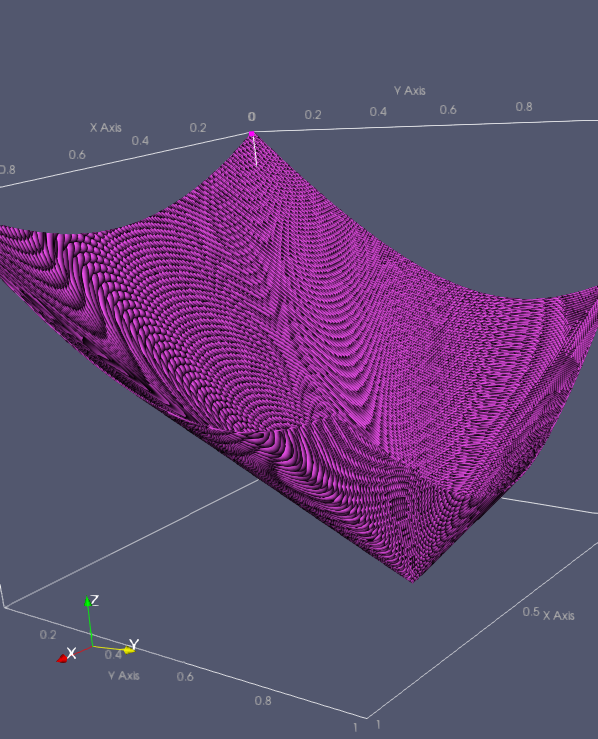
\includegraphics[width=0.25\linewidth]{görüntü_1.png}
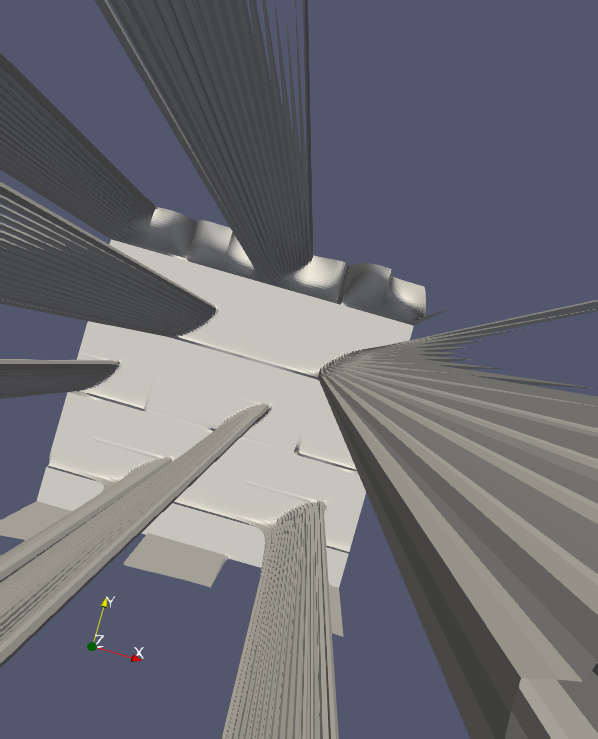
\includegraphics[width=0.25\linewidth]{görüntü_2.png}
\caption{\label{fig:time step 0}This images were created using Paraview.}
\end{figure}
We understand that the last time step image is somewhat different than the one on the homework. We hope for further help with those files from fellow collaborators and our instructors.

\end{document}